\chapter{Plano de cableado vertical}
\section{Distribuidores etiquetados. Dentro de cada distribuidor detallar gráficamente los dispositivos instalados}
\begin{center}
	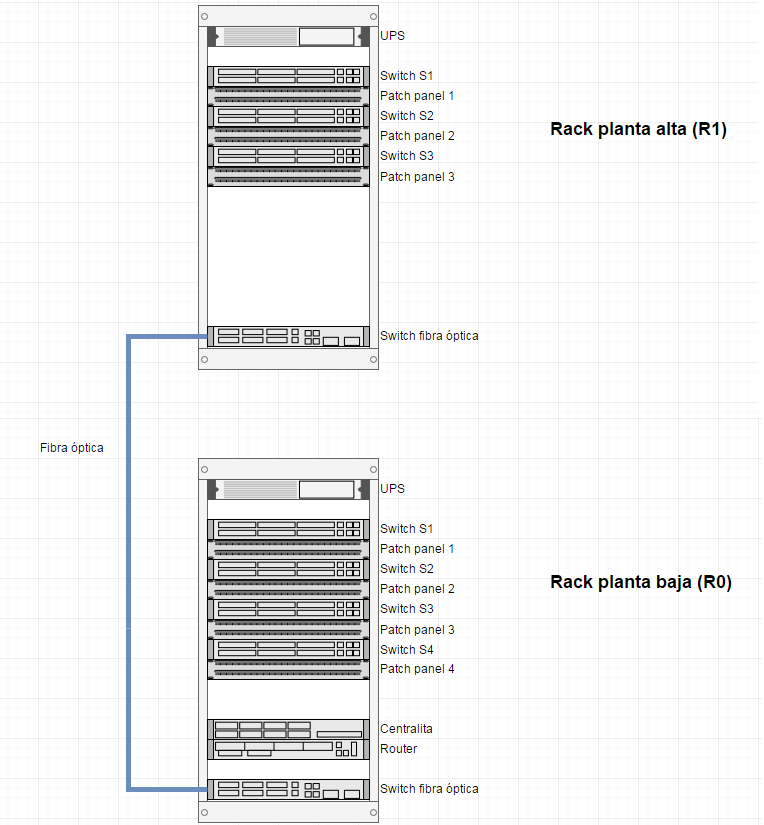
\includegraphics[scale=0.65]{CV.png}
\end{center}
\newpage
Tal como podemos ver en la imagen, el Rack 0 se encontraría en la planta baja y contaría con los siguientes dispositivos:
\begin{itemize}
	\item Una UPS (sistema de alimentación ininterrumpida = SAI).
	\item Cuatro switches con tecnología PoE para suministro eléctrico en caso de ser necesario en teléfonos VoIP o puntos de acceso. Estos switches también cuentan con puertos de fibra óptica.
	\item Cuatro patch panels.
	\item Una centralita telefónica.
	\item Un router.
	\item Un switch de fibra óptica exclusivo para cableado vertical.
\end{itemize}
El Rack 0 (planta baja) está conectado con el Rack 1 (planta alta) mediante fibra óptica multimodo. El Rack 1 cuenta con los siguientes dispositivos:
\begin{itemize}
	\item Una UPS (sistema de alimentación ininterrumpida = SAI).
	\item Tres switches con tecnología PoE para suministro eléctrico en caso de ser necesario en teléfonos VoIP o puntos de acceso. Estos switches también cuentan con puertos de fibra óptica.
	\item Tres patch panels.
	\item Un switch de fibra óptica exclusivo para cableado vertical.
\end{itemize}